\subsection{Value Model}

The $e3$ value model represents how actors exchange value by providing services.
The $e3$ value model helps business understand the dependencies and interactions between
the value proposition, value configuration, and value network.

\begin{itemize}
    \item \textbackslash Courier Accepts orders from a platform/app published by clients and goes to the storage to get the necessary items. Courier ships the order to a client and proceeds with the next order.
    \item \textbackslash Customer Uses a platform/app to combine the order and pays for it. After waiting for a delivery, a customer collects the order from a courier.
    \item \textbackslash Platform/App Is used by a client to share the information about items in a stock and the information about the order. Platform / App is used by a courier to show the list of available orders and communicate with a customer. The app navigates a courier inside the storage and outside on the way to a customer’s location.
    \item \textbackslash Storage The items are stored in a storage that gives the access to couriers to complete the order. The items in a storage are supplied from a goods provider.
    \item \textbackslash Goods Provider Sends products to a storage and gets money from the delivery company.
\end{itemize}

\subsection{Value Model Diagram}

Value model diagram provides a visual representation of how value is created, delivered, and captured within a business context.

\begin{figure}[H]
	\centering
	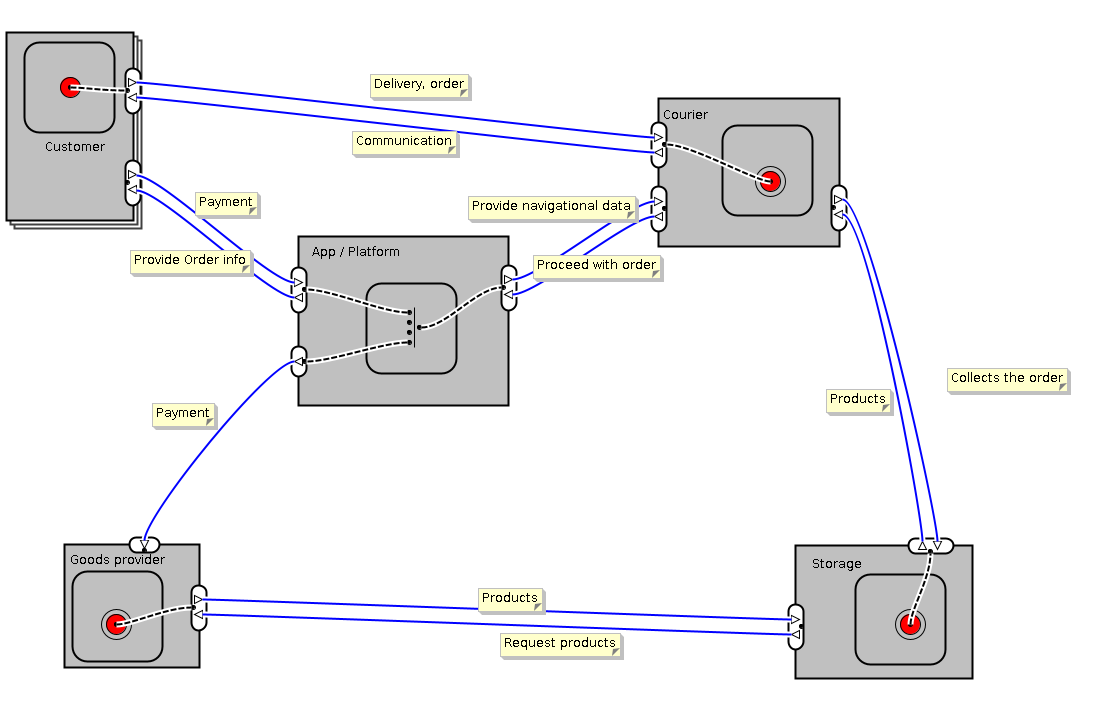
\includegraphics[width=14cm]{value_model}
	\caption{Value Model}
	\label{fig:value_model}
\end{figure}
